\section{Results}
\label{sec:results}

In this section we present numerical results for the NLO QCD and NLO EW 
corrections to all three production processes of a diphoton pair in 
association with a third vector boson, a third photon, a $W$ or a $Z$ 
boson, at the LHC at a centre-of-mass energy of 13\,TeV. 
In case of an accompanying $W$ or a $Z$ boson, we consider the full 
off-shell leptonic final state, i.e.\ lepton-neutrino or lepton-pair 
production.
All results are obtained in the Standard Model using the complex-mass 
scheme \cite{Denner:2005fg} with the following input parameters
\begin{center}
  \begin{tabular}{rclrcl}
    $\alphazero$ &\shortequal& $1/137.03599976$  \qquad &&& \\
    $G_\mu$ &\shortequal& $1.1663787\times 10^{-5}\; \text{GeV}^2$ &&& \\
    $m_W$ &\shortequal& $80.385\; \text{GeV}$       & $\Gamma_W$ &\shortequal& $2.085\; \text{GeV}$ \\
    $m_Z$ &\shortequal& $91.1876\; \text{GeV}$      & $\Gamma_Z$ &\shortequal& $2.4952\; \text{GeV}$ \\
    $m_h$ &\shortequal& $125.0\; \text{GeV}$        & $\Gamma_h$ &\shortequal& $0$\\
    $m_t$ &\shortequal& $173.2\; \text{GeV}$        & $\Gamma_t$ &\shortequal& $0$\;.
  \end{tabular}
\end{center}
Both the width of the top quark and the Higgs boson can safely be 
neglected as there are no diagrams containing either as $s$-channel 
propagators which can potentially go on-shell. 
All other lepton and parton masses and widths are set to zero, 
i.e.\ we are working in the five-flavour scheme.
We use the \textsc{CT14nlo} PDF set with $\alphas(m_Z)=0.118$. 
The use of a QCD-only PDF is justified by the fact that, 
at LO, the photon induced corrections are either non-existant 
(\aaa, \aaw) or negligible (\aaz).
This finding will be detailed in Section \ref{sec:results:aaz}.

We define our central scales through
\begin{equation}
  \label{eq:murfdef}
  \begin{split}
    \muR^0 = \muF^0 = \left\{
    \begin{array}{ll}
      m_{\aaa} \qquad & \text{in \aaa\ production} \\[2mm]
      \tfrac{1}{2}\,H_T' & \text{in \aaw\ and \aaz\ production.}
    \end{array}\right.
  \end{split}
\end{equation}
Therein, the modified scalar sum of transverse momenta is defined as 
\begin{equation}
  \label{ew:defHT}
  \begin{split}
    H_\mathrm{T}' = E_\mathrm{T}^V + \sum_{\gamma,q,g} p_{\mathrm{T},i}
  \end{split}
\end{equation}
with $\left.E_\mathrm{T}^W\right.^2=(p_\ell+p_\nu)^2$ and 
$\left.E_\mathrm{T}^Z\right.^2=(p_{\ell^+}+p_{\ell^-})^2$ 
in full analogy to the case of the case of vector boson production 
in association with jets \cite{}.
As the Born process in each case has no $\muR$ dependence, we 
do not expect the choice of scale to have a significant influence 
on the size of the relative QCD and EW corrections.
We calculate $\mathrm{B}(\muF)$, $\deltaQCD(\muR,\muF)$ and 
$\deltaEW(\muF^0)$ and vary the free scales $\muR$ and $\muF$ 
by the conventional factor of two around their central values 
$\muR^0$ and $\muF^0$, respectively.
We do not vary the factorisation scale for the determination 
of $\deltaEW$ as the inherent, albeit normally phenomenologically 
irrelevant, stabilisation of the $\muF$-dependence at NLO EW 
is not reflected in our chosen PDF.
Hence, our NLO EW result exhibits the exact same $\muF$-dependence 
as the LO result.


\begin{table}[t!]
  \centering
  \begin{tabular}{l||c|c|c}
      & $\;\;pp \to \gamma \gamma\gamma\;\;$
      & $\;\;pp \to \gamma \gamma e^-\bar\nu_e\;\;$ 
      & $\;\;pp \to \gamma \gamma e^+e^-\;\;$ \\
    \hline\hline
    $\sigma_\text{LO}\;\;[\text{pb}] $ &  &  & \\
    \hline
    $\delta_\text{QCD}\;\;[\text{pb}]\;\;\pTveto=\infty $ &  &  & \\
    \hline
    $\delta_\text{QCD}\;\;[\text{pb}]\;\;\pTveto=30\,\text{GeV} $ &  &  & \\
    \hline
    $\delta_\text{EW}\;\;[\text{pb}] $ &  &  & \\
  \end{tabular}
  \caption{
    Total cross sections at LO, NLO QCD and NLO EW for $\gamma\gamma\gamma$, 
    $\gamma\gamma e^-\bar\nu_e$ and $\gamma\gamma e^+e^-$
    production at 13\,TeV at the LHC.
    \label{tab:xsec}
  } 
\end{table}


\subsection[\texorpdfstring{$\gamma\gamma\gamma$}{aaa} production]
           {$\boldsymbol{\gamma\gamma\gamma}$ production}
\label{sec:results:aaa}

\begin{figure}[t!]
  \centering
  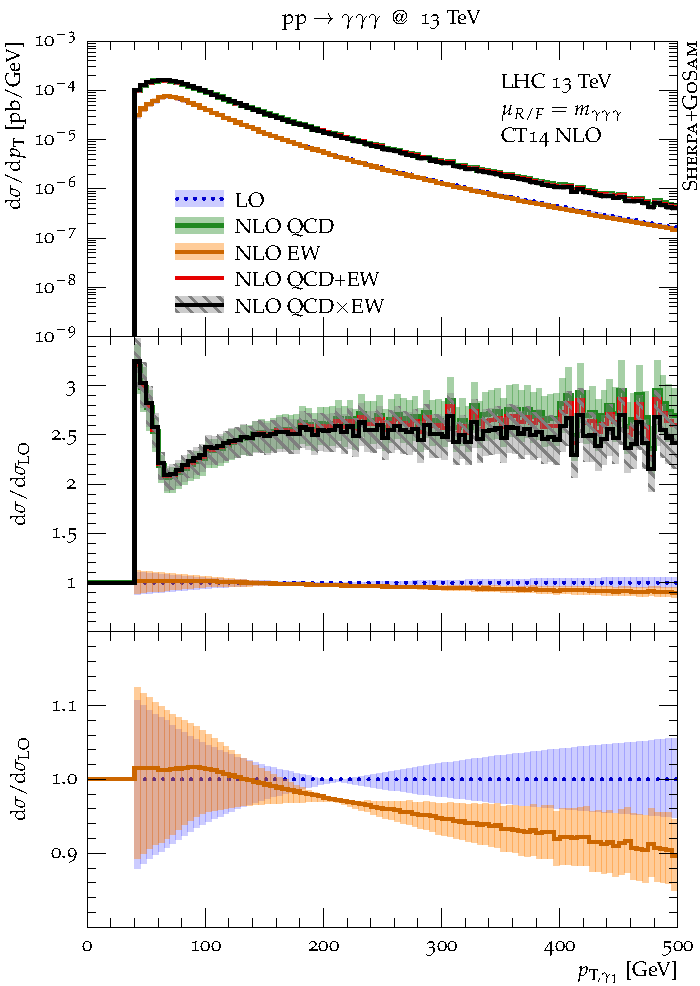
\includegraphics[width=0.32\textwidth]{figs_aaa/pT_y1}
  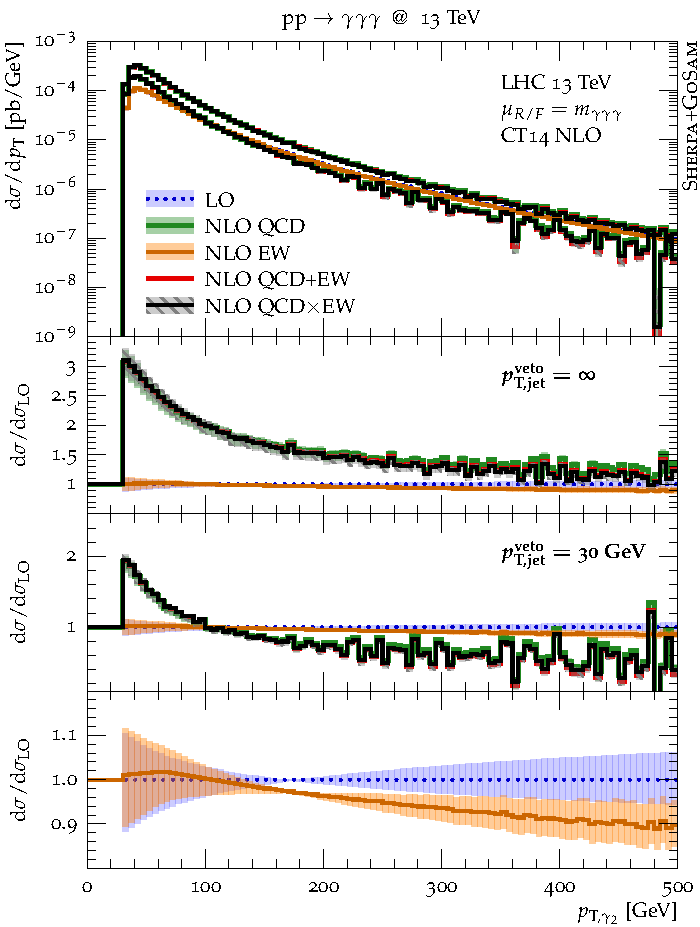
\includegraphics[width=0.32\textwidth]{figs_aaa/pT_y2}
  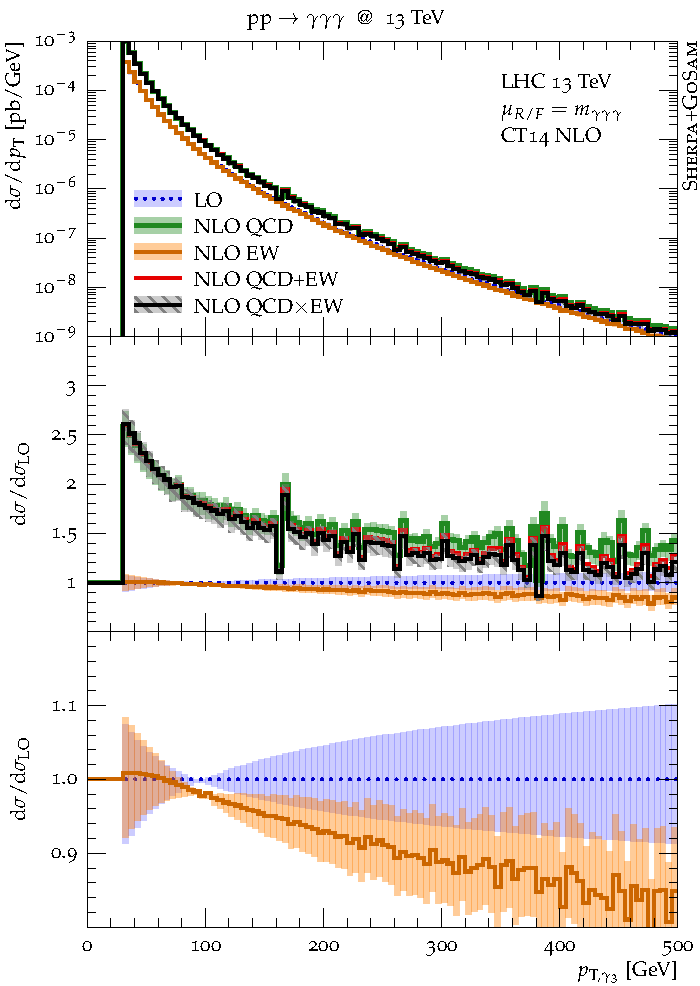
\includegraphics[width=0.32\textwidth]{figs_aaa/pT_y3}
  \caption{
    Transverse momentum of the leading (left), subleading (centre) 
    and third leading (right) photon 
    in triple photon production at the LHC at 13\,TeV. 
    The distributions are shown at LO (blue), NLO QCD (green), 
    NLO EW (orange), NLO \QCDpEW\ (red) and NLO \QCDtEW\ (black) 
    including scale uncertainties. The top ratio plot details 
    the relative corrections to the leading order cross section 
    without applying any jet veto, while the centre ratio plot 
    applies a jet veto of $p_\mathrm{T,jet}^\mathrm{veto}=\text{30\,GeV}$. 
    The lower ratio highlights the size of the electroweak corrections.
    \label{fig:aaa:pt}
  }
\end{figure}

\begin{figure}[t!]
  \centering
  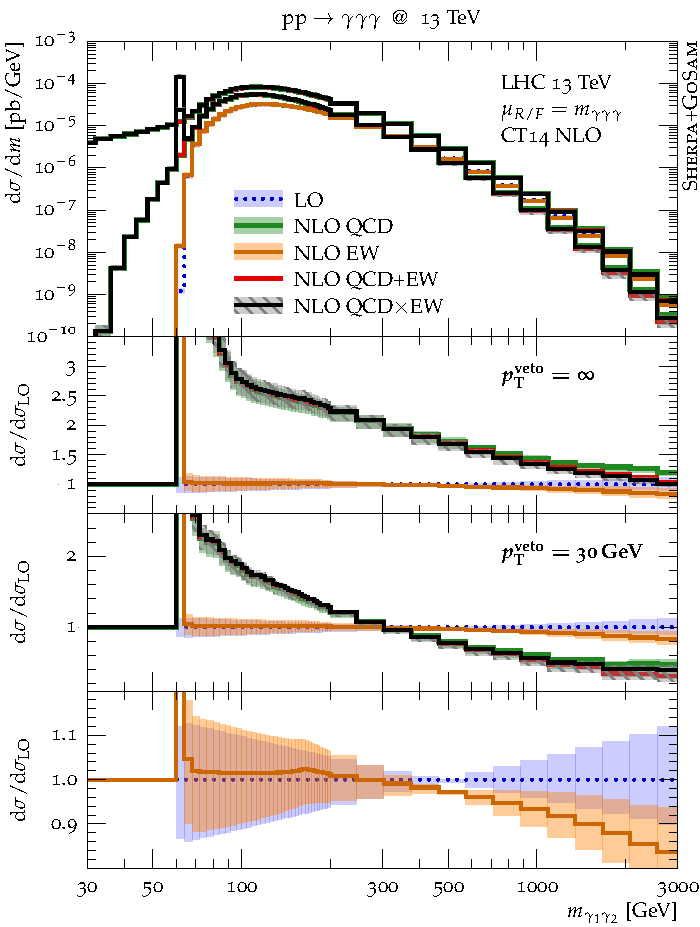
\includegraphics[width=0.32\textwidth]{figs_aaa/m_y1y2_comb_log}
  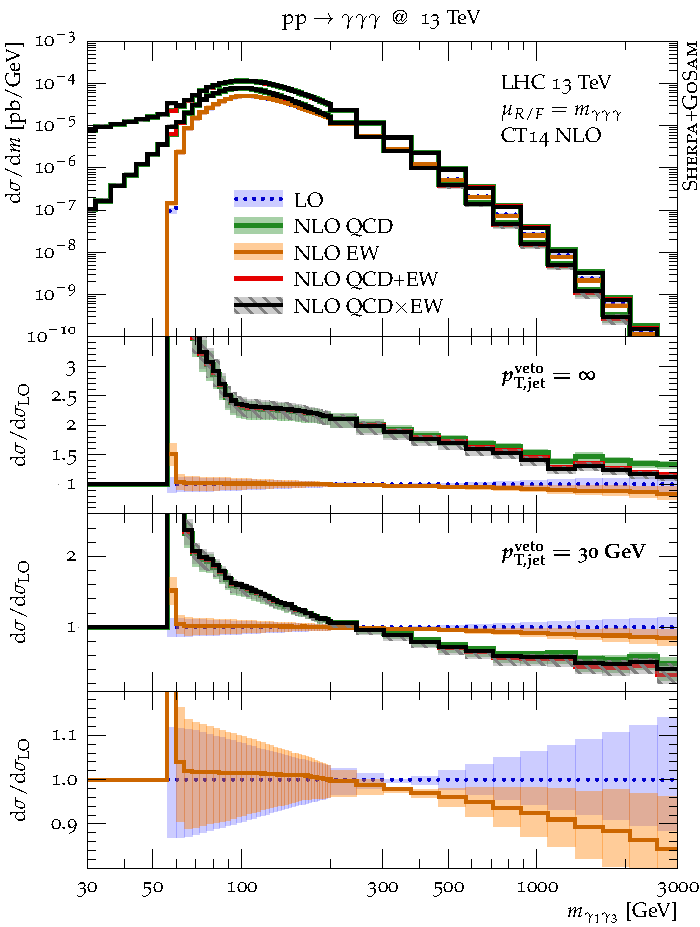
\includegraphics[width=0.32\textwidth]{figs_aaa/m_y1y3_comb_log}
  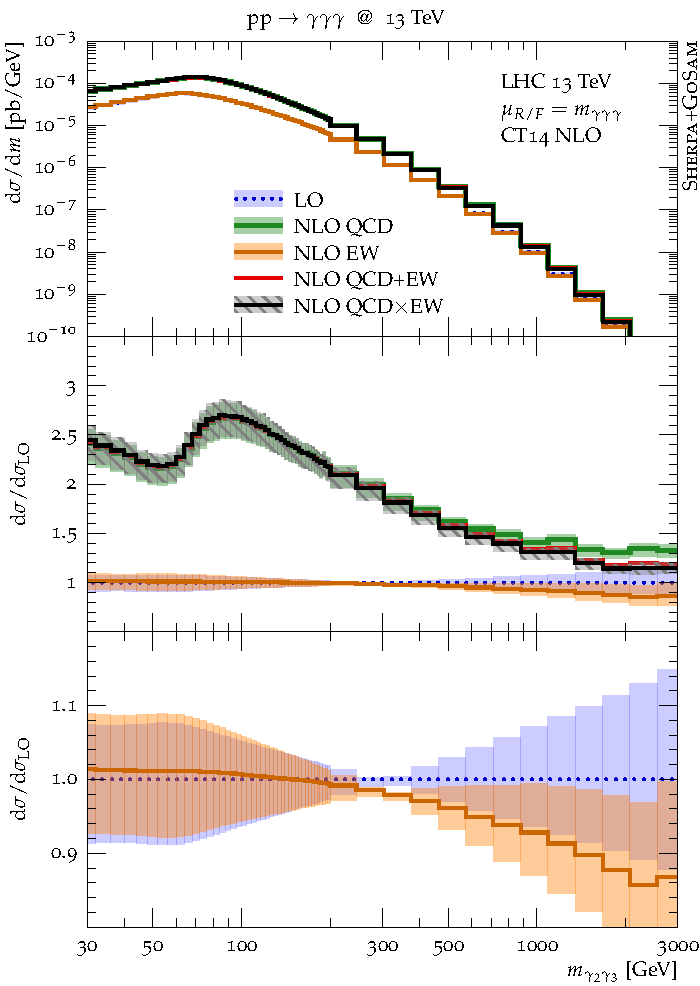
\includegraphics[width=0.32\textwidth]{figs_aaa/m_y2y3_comb_log}
  \caption{
    Pairwise invariant mass of the leading and subleading photon (left),
    leading and third leading photon (centre), subleading and third leading 
    photon (right) 
    in triple photon production at the LHC at 13\,TeV. 
    Details as in Fig.\ \ref{fig:aaa:pt}.\\
    \comment{MS: Spike in $m_{\gamma_1\gamma_2}$ is in NLO \QCDtEW\ 
             and comes from $\deltaEW\approx 10$ in this bin at the 
             edge of the LO phase space.}
    \label{fig:aaa:myy}
  }
\end{figure}

\begin{figure}[t!]
  \centering
  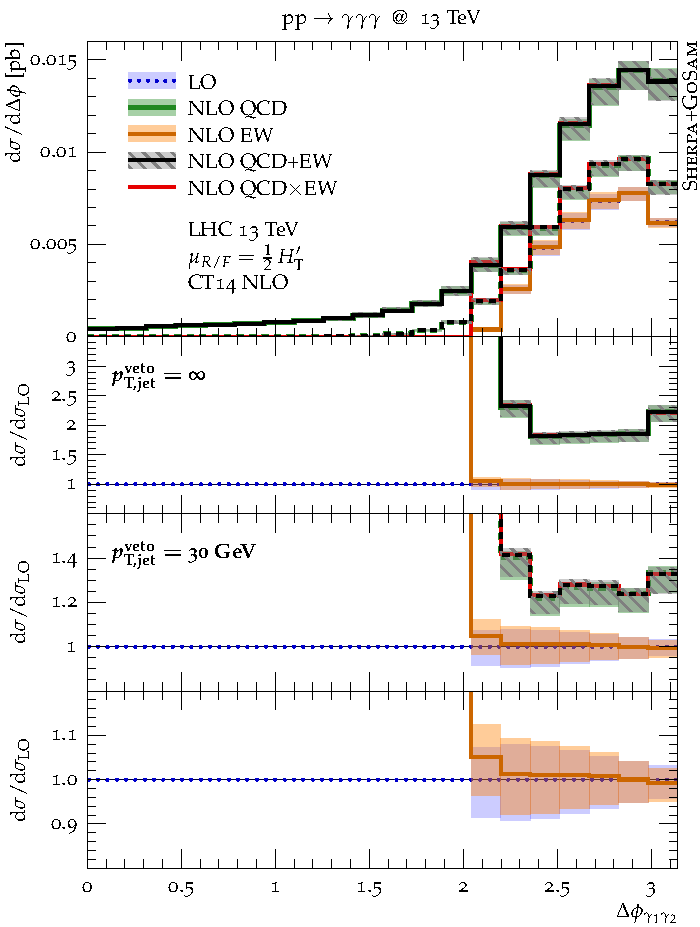
\includegraphics[width=0.32\textwidth]{figs_aaa/dphi_y1y2}
  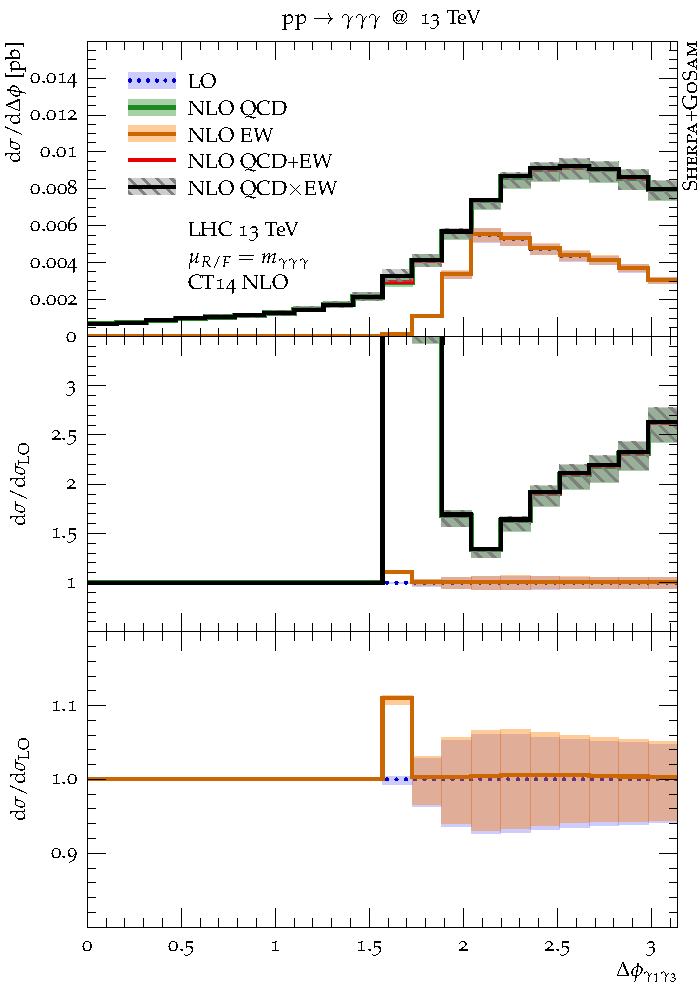
\includegraphics[width=0.32\textwidth]{figs_aaa/dphi_y1y3}
  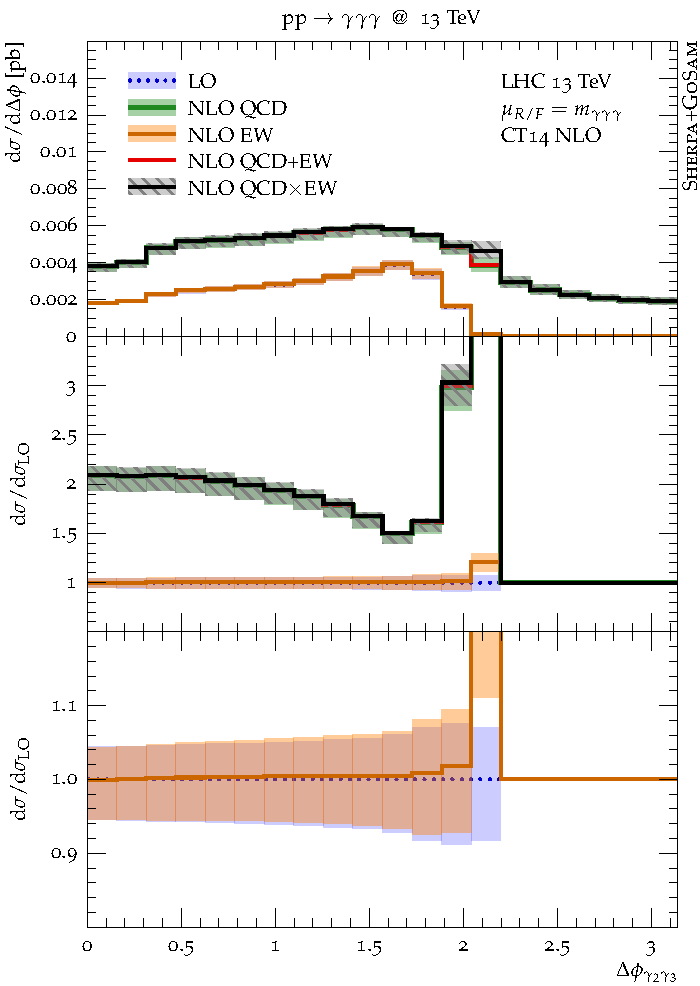
\includegraphics[width=0.32\textwidth]{figs_aaa/dphi_y2y3}
  \caption{
    Azimuthal separation of the leading and subleading photon (left),
    leading and third leading photon (centre), subleading and third leading 
    photon (right) 
    in triple photon production at the LHC at 13\,TeV. 
    Details as in Fig.\ \ref{fig:aaa:pt}.\\
    \comment{MS: Spike in $\Delta\phi_{\gamma_2\gamma_3}$ is in NLO \QCDtEW\ 
             and comes from $\deltaEW\approx 2$ in this bin at the 
             edge of the LO phase space.}
    \label{fig:aaa:dphi}
  }
\end{figure}

\begin{itemize}
  \item \pT of 3rd photon much softer than 1st and 2nd
  \item EW corrections to \pT of 1st and 2nd photon nearly identical and 
        $\approx -10\%$ at 500\,GeV, 3rd photon almost twice that.
  \item in all cases NLO EW outside LO uncertainty band
  \item NLO QCD dominated by real corrections, i.e.\ additional 
        jet emissions
  \item intensified through opening of new $qg$ channels and large 
        gluon luminosity
  \item can be controlled in fixed-order calculations through jet veto, 
        needs proper multijet merging
  \item because at LO the leading jet needs to be in the opposite 
        hemisphere as the subleading and third leading jet, 
        $m_{\gamma_1\gamma_2}$ and $m_{\gamma_1\gamma_3}$ 
        exhibit kinematic edges at LO
  \item kinematic conditions relaxed at NLO (both QCD and EW, 
        but QCD dominating), large corrections around those edges, 
        leads to artifacts in multiplicative combination
  \item NLO QCD very similar for $m_{\gamma_1\gamma_2}$ and 
	$m_{\gamma_1\gamma_3}$, $m_{\gamma_2\gamma_3}$ with interesting 
	structure around 80-90\,GeV
  \item $m_{\gamma_1\gamma_2}$ again exhibits small excess at $2m_W$
  \item small positive EW corrections at small $m_{\gamma\gamma}$ 
  \item $\approx -10\%$ at 1\,TeV for all $m_{\gamma\gamma}$ 
  \item NLO EW very similar for all $m_{\gamma\gamma}$ 
\end{itemize}



\subsection[\texorpdfstring{$\gamma\gamma\ell\nu$}{aalnu} production]
           {$\boldsymbol{\gamma\gamma\ell\nu}$ production}
\label{sec:results:aaw}

\comment{MS: is that $\ell^+$ or $\ell^-$?}

\begin{figure}[t!]
  \centering
  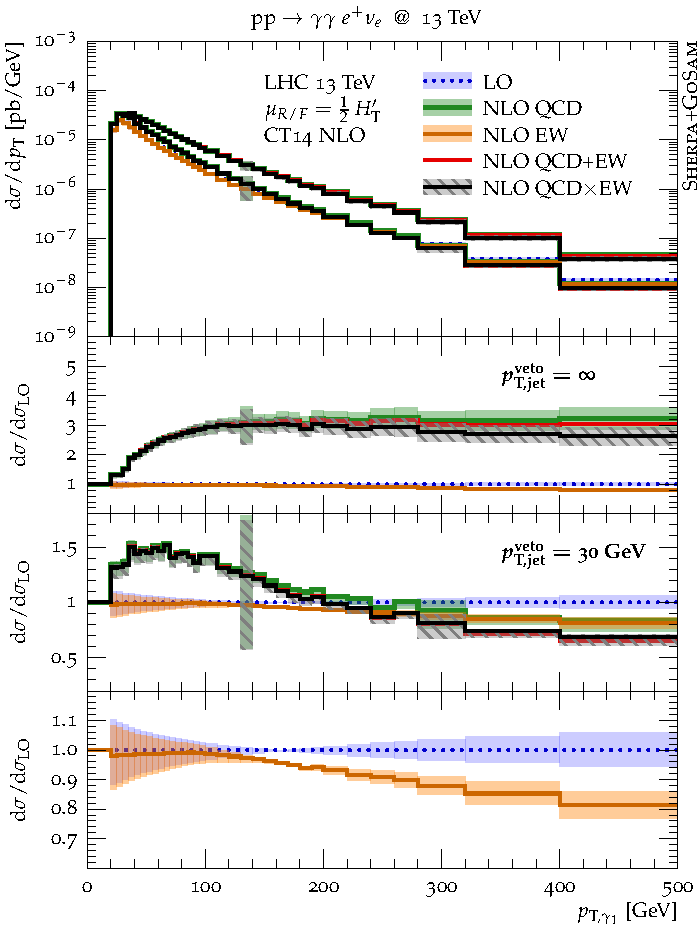
\includegraphics[width=0.32\textwidth]{figs_aaw/pT_y1}
  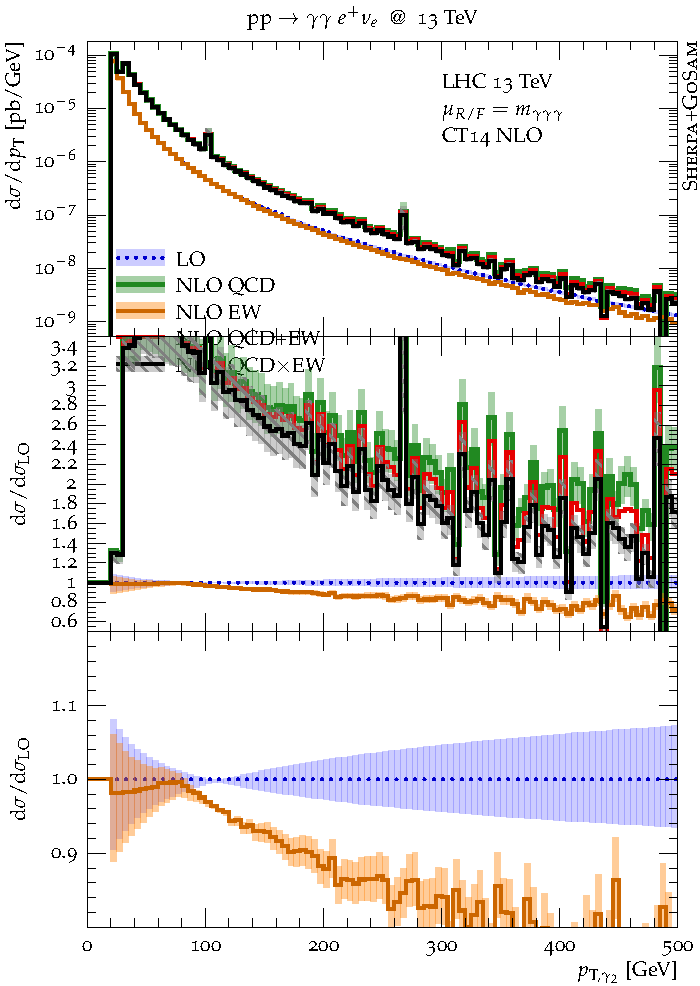
\includegraphics[width=0.32\textwidth]{figs_aaw/pT_y2}
  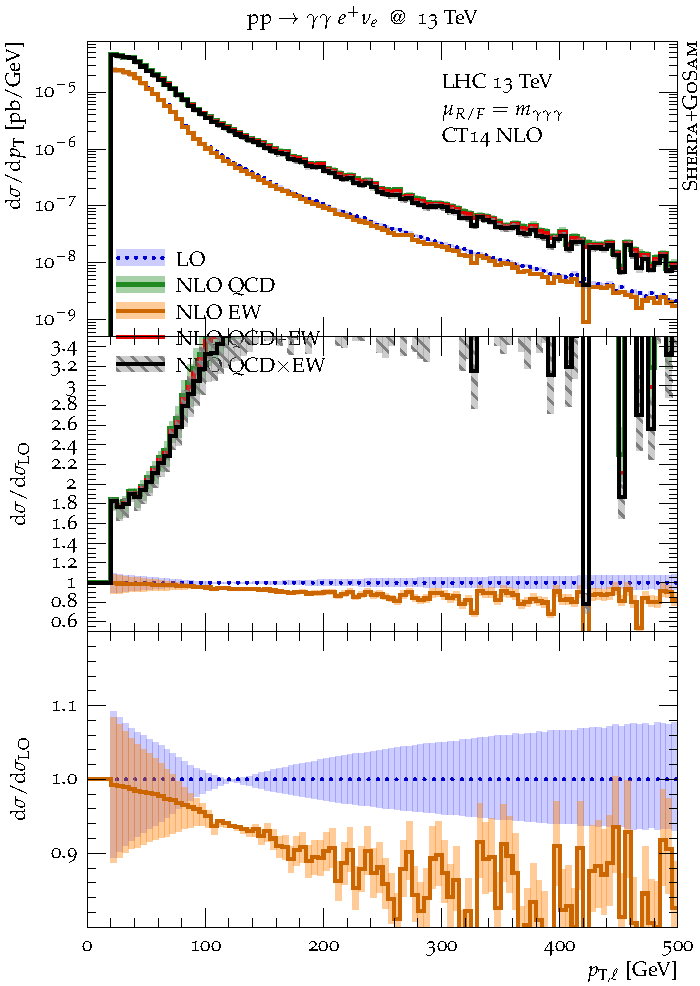
\includegraphics[width=0.32\textwidth]{figs_aaw/pT_l1}
  \caption{
    Transverse momentum of the leading (left), subleading (centre) 
    and third leading (right) photon at the LHC at 13\,TeV.
    \label{fig:aaw:pt}
  }
\end{figure}

\begin{figure}[t!]
  \centering
  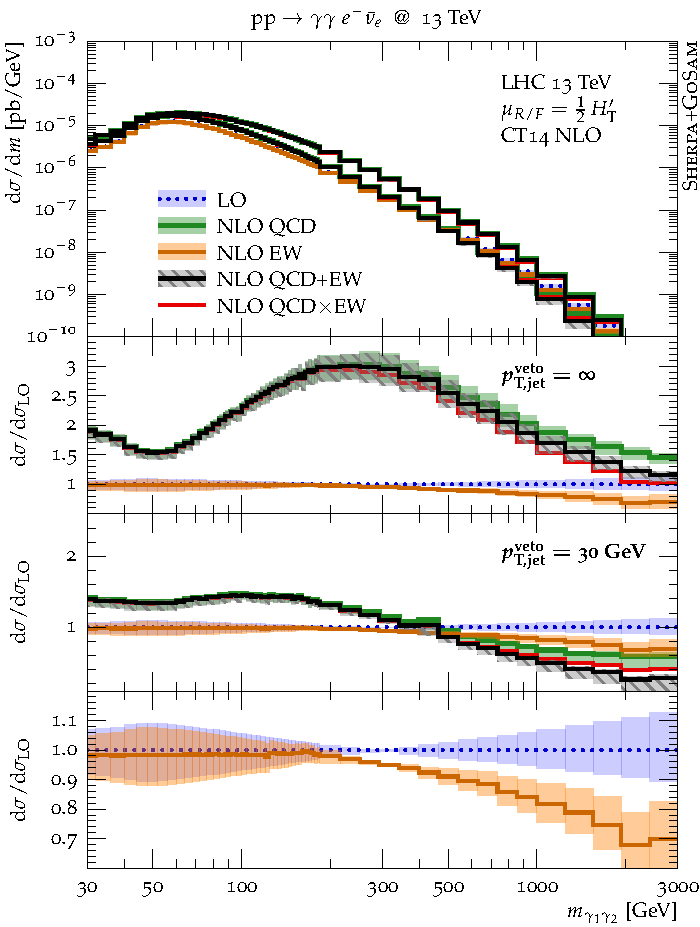
\includegraphics[width=0.32\textwidth]{figs_aaw/m_y1y2_comb_log}
  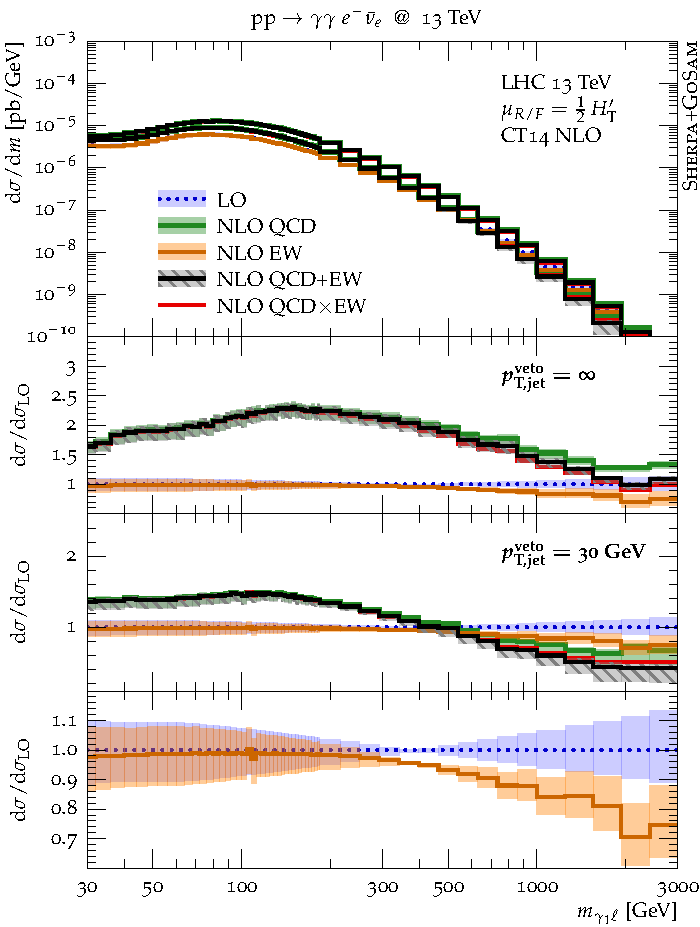
\includegraphics[width=0.32\textwidth]{figs_aaw/m_y1l1_comb_log}
  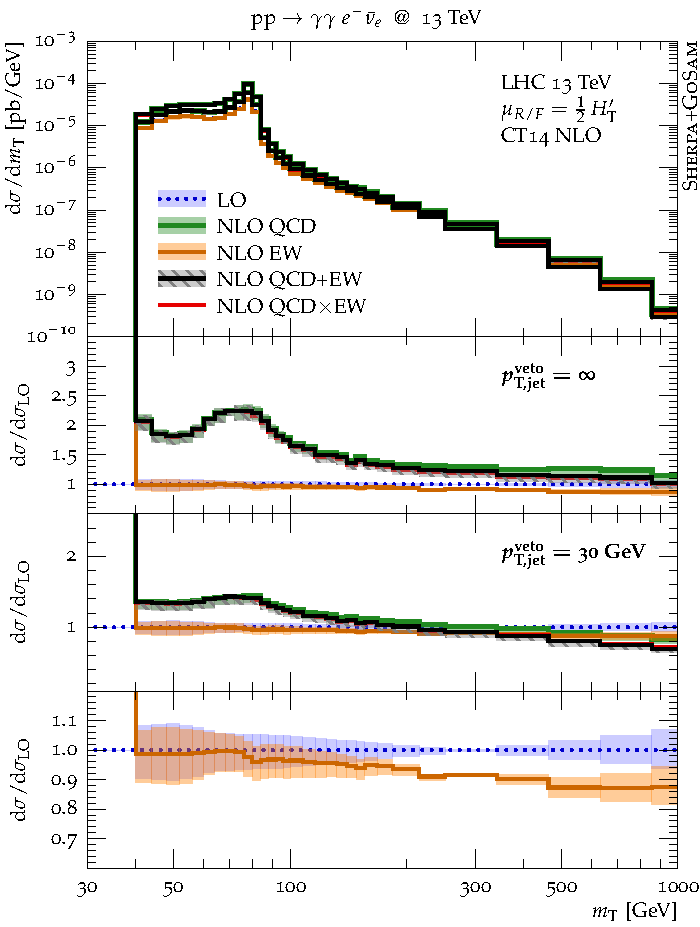
\includegraphics[width=0.32\textwidth]{figs_aaw/m_t_comb_log}
  \caption{
    Pairwise invariant mass of the leading and subleading photon (left),
    leading and third leading photon (centre), subleading and third leading 
    photon (right) at the LHC at 13\,TeV.\\
    \comment{MS: Spike in $m_{\gamma_1\gamma_2}$ is in NLO \QCDtEW 
             and comes from $\deltaEW\approx 10$ in this bin at the 
             edge of the LO phase space.}
    \label{fig:aaw:myy}
  }
\end{figure}

\begin{figure}[t!]
  \centering
  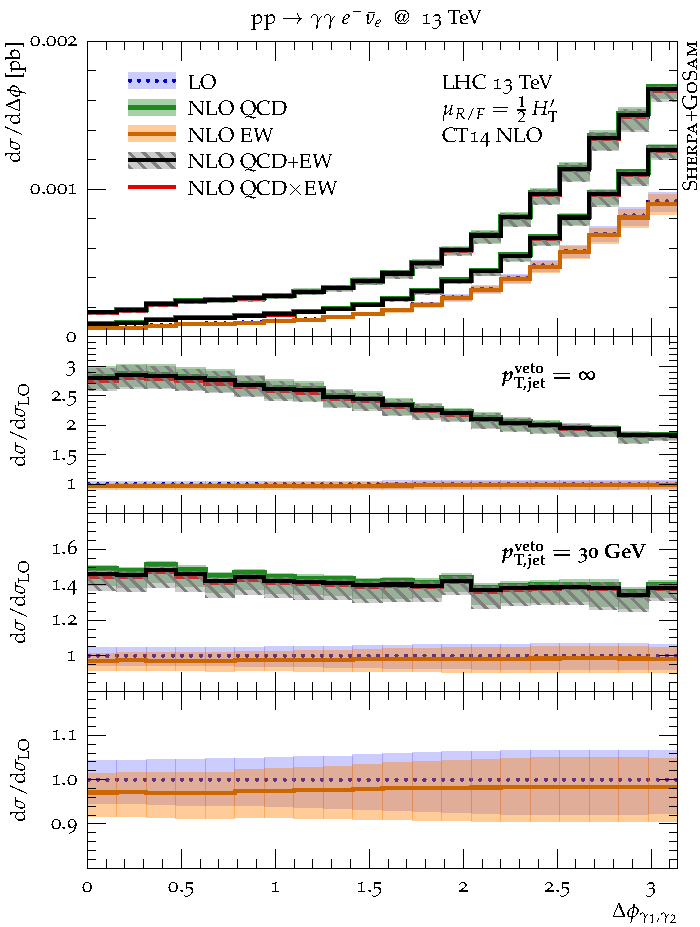
\includegraphics[width=0.32\textwidth]{figs_aaw/dphi_y1_y2}
  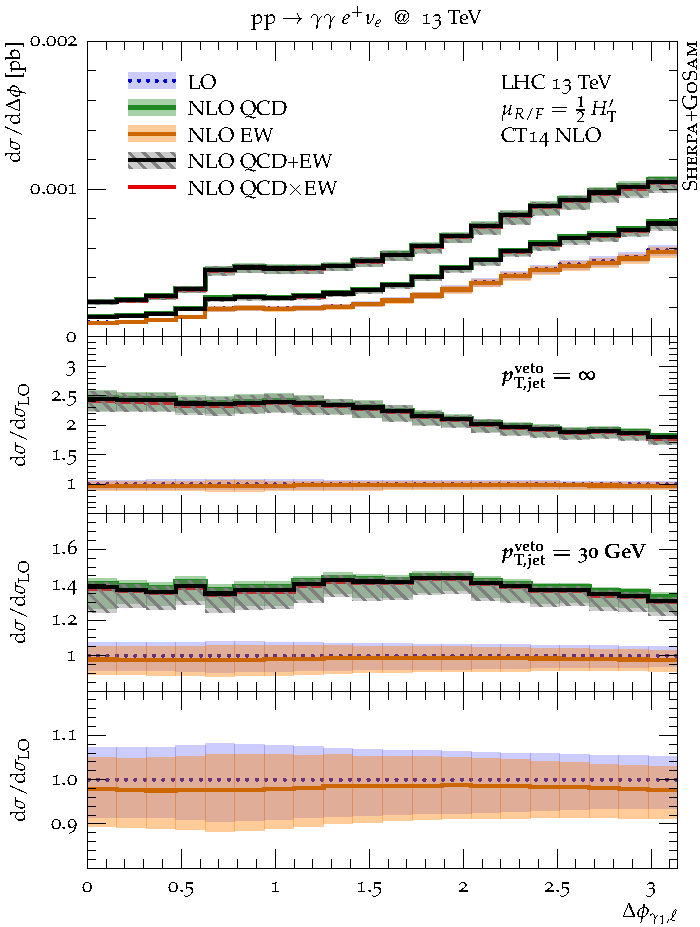
\includegraphics[width=0.32\textwidth]{figs_aaw/dphi_y1_l1}
  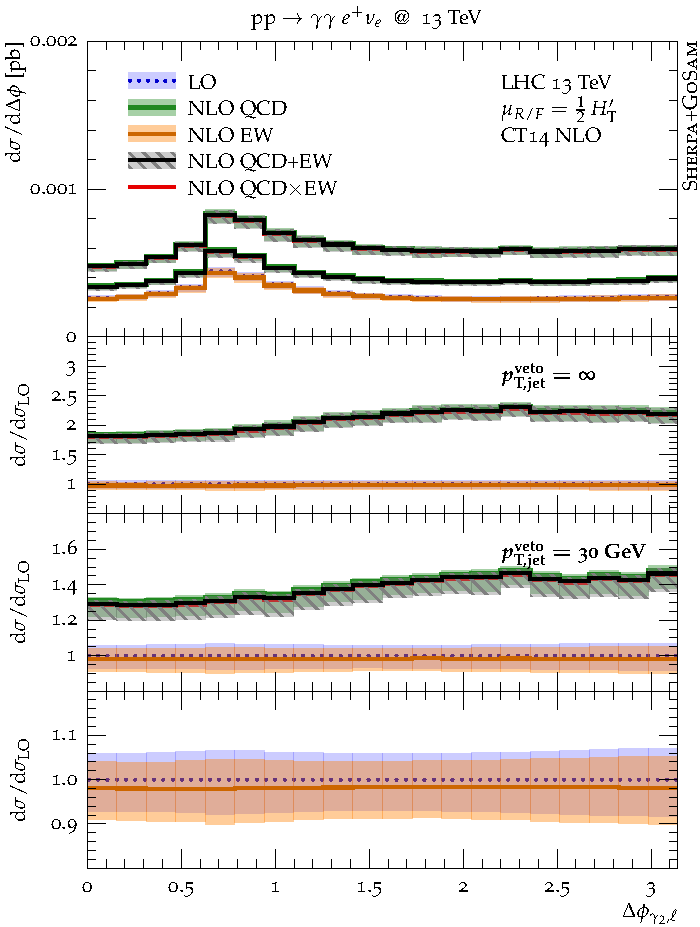
\includegraphics[width=0.32\textwidth]{figs_aaw/dphi_y2_l1}
  \caption{
    Azimuthal separation of the leading and subleading photon (left),
    leading and third leading photon (centre), subleading and third leading 
    photon (right) at the LHC at 13\,TeV.\\
    \comment{MS: Spike in $m_{\gamma_1\gamma_2}$ is in NLO \QCDtEW 
             and comes from $\deltaEW\approx 10$ in this bin at the 
             edge of the LO phase space.}
    \label{fig:aaw:dphi}
  }
\end{figure}


\subsection[\texorpdfstring{$\gamma\gamma\ell^+\ell^-$}{aall} production]
           {$\boldsymbol{\gamma\gamma\ell^+\ell^-}$ production}
\label{sec:results:aaz}

\begin{figure}[t!]
  \centering
  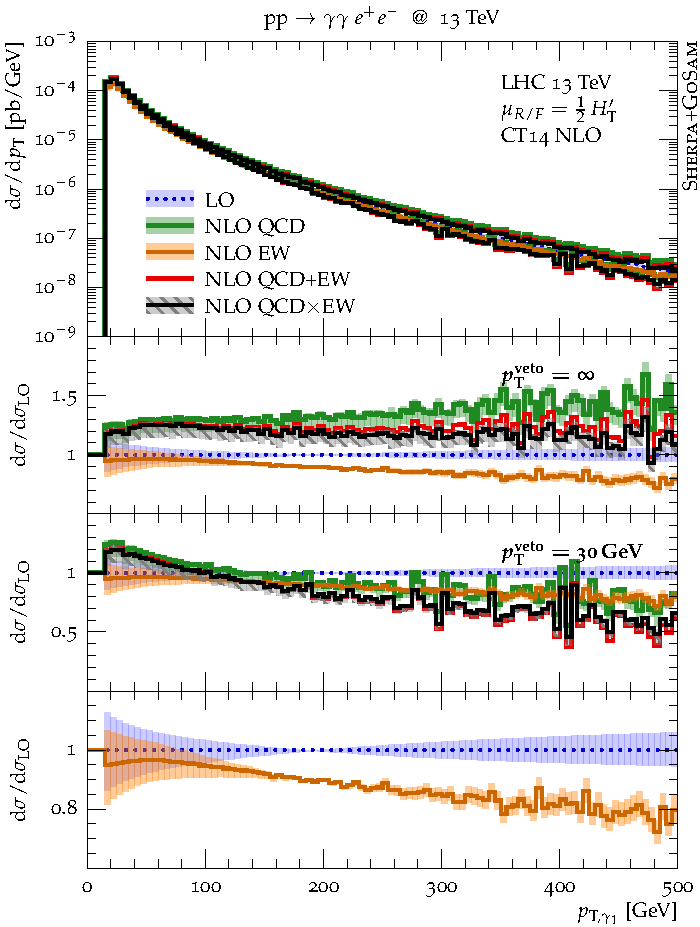
\includegraphics[width=0.32\textwidth]{figs_aaz/pT_y1}
  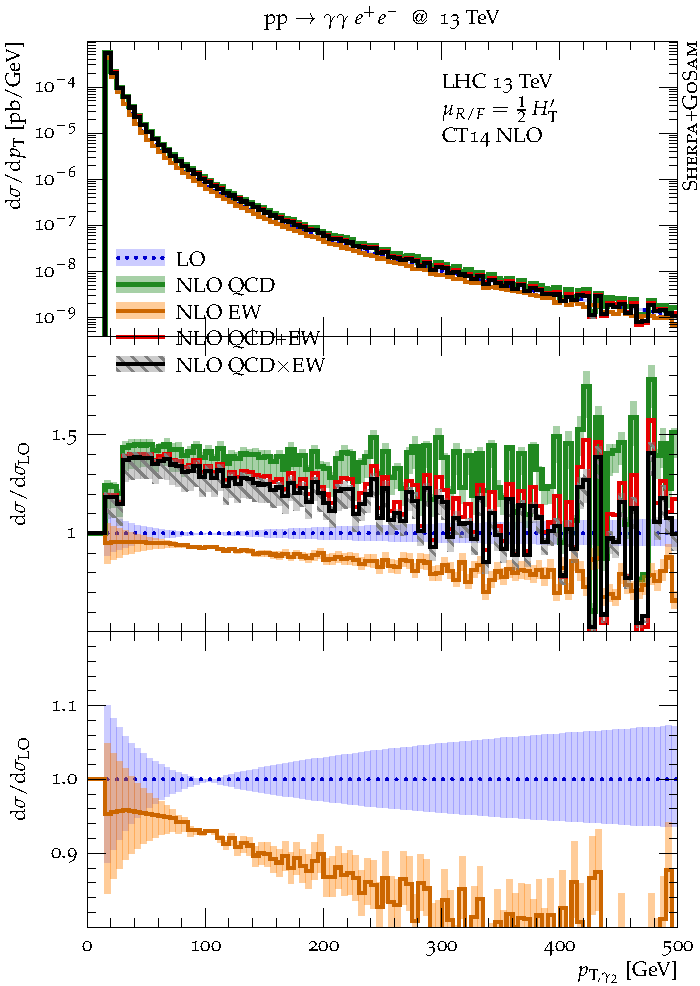
\includegraphics[width=0.32\textwidth]{figs_aaz/pT_y2}
  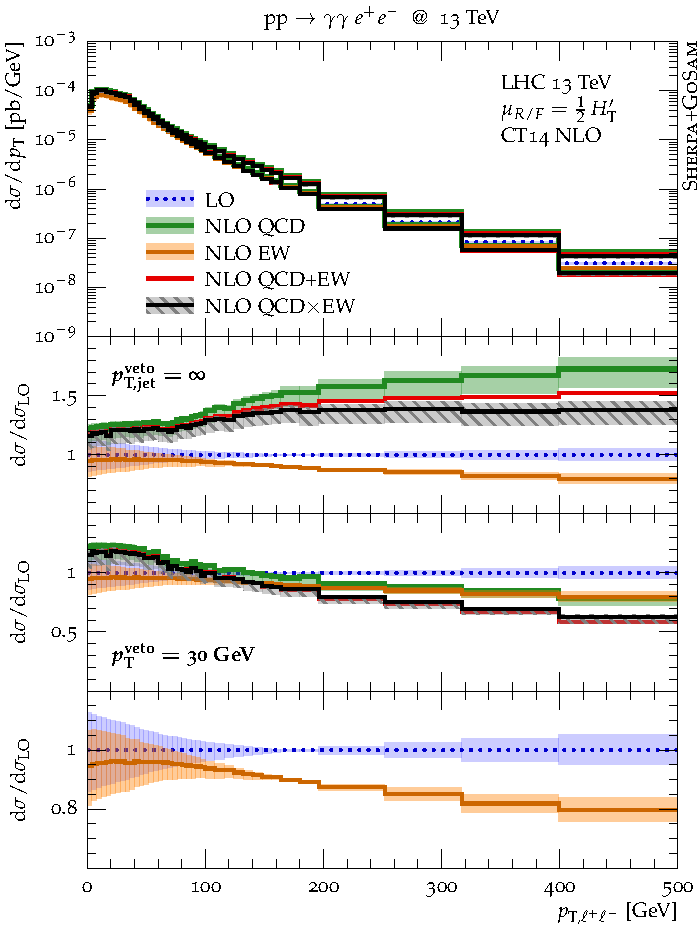
\includegraphics[width=0.32\textwidth]{figs_aaz/pT_l1l2_comb_log}
  \caption{
    Transverse momentum of the leading (left) and subleading (centre) 
    photon as well as the dressed lepton pair (right) 
    in diple photon production in association with a lepton pair 
    at the LHC at 13\,TeV. 
    Details as in Fig.\ \ref{fig:aaa:pt}.
    \label{fig:aaz:pt}
  }
\end{figure}

\begin{figure}[t!]
  \centering
  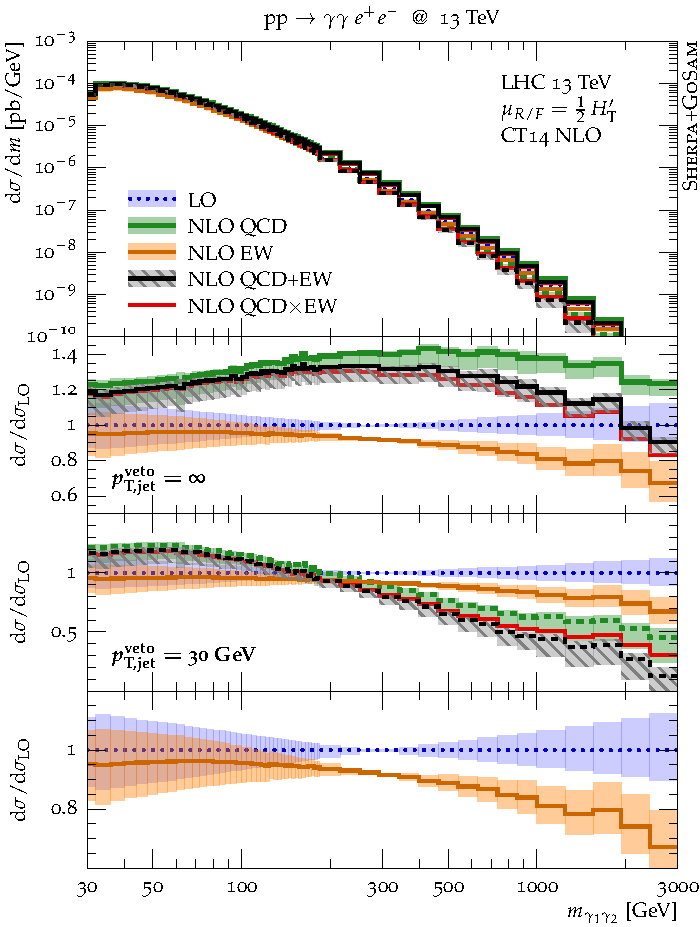
\includegraphics[width=0.32\textwidth]{figs_aaz/m_y1y2_comb_log}
  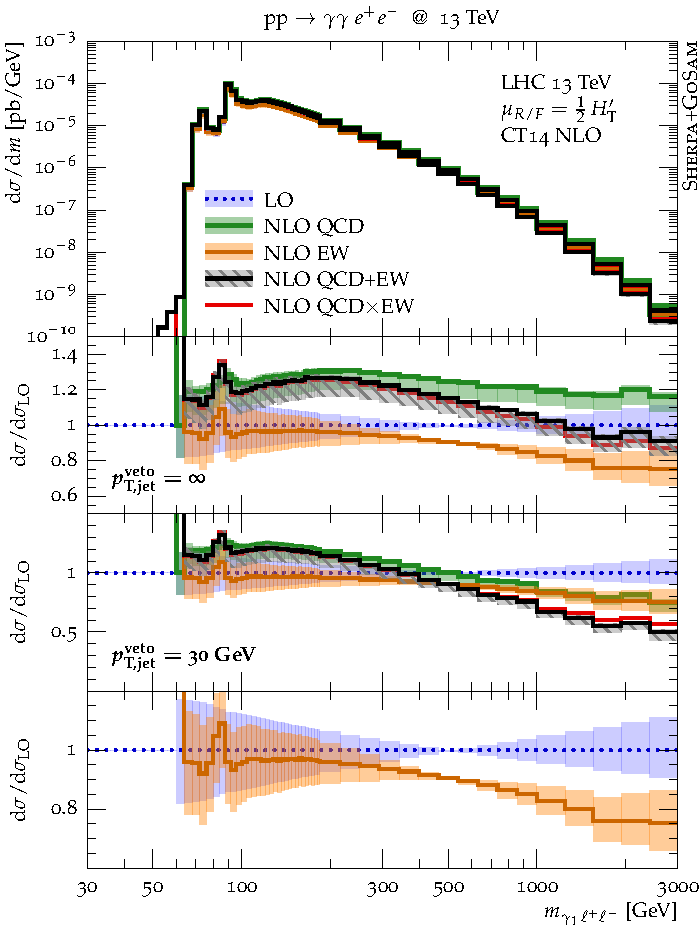
\includegraphics[width=0.32\textwidth]{figs_aaz/m_y1l1l2_comb_log}
  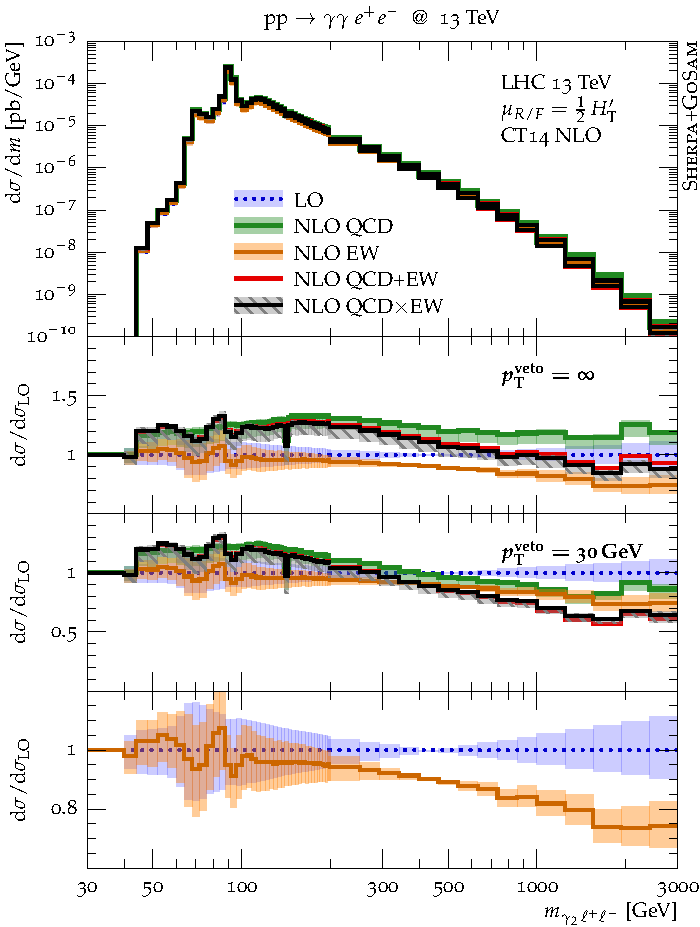
\includegraphics[width=0.32\textwidth]{figs_aaz/m_y2l1l2_comb_log}
  \caption{
    Pairwise invariant mass of the leading and subleading photon (left),
    the leading photon and the lepton pair (centre), and the subleading 
    photon and the lepton pair (right)
    in diple photon production in association with a lepton pair 
    at the LHC at 13\,TeV. 
    Details as in Fig.\ \ref{fig:aaa:pt}.\\
    \comment{MS: Spike in $m_{\gamma_1\ell_1\ell_2}$ is in NLO \QCDtEW\ 
             and comes from $\deltaEW\approx 10$ in this bin at the 
             edge of the LO phase space.}
    \label{fig:aaz:myy}
  }
\end{figure}

\begin{figure}[t!]
  \centering
  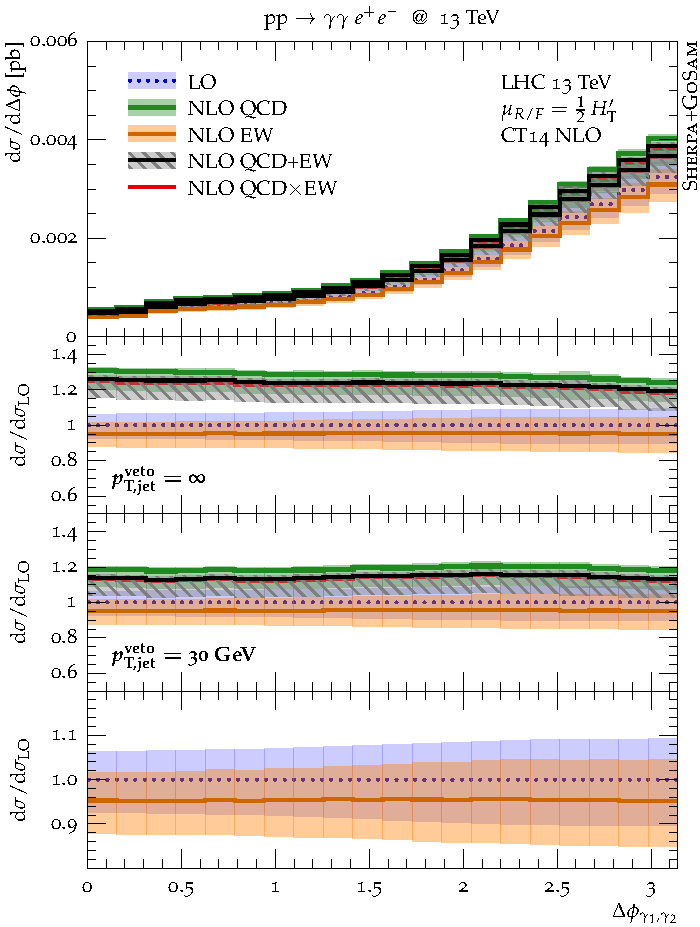
\includegraphics[width=0.32\textwidth]{figs_aaz/dphi_y1_y2}
  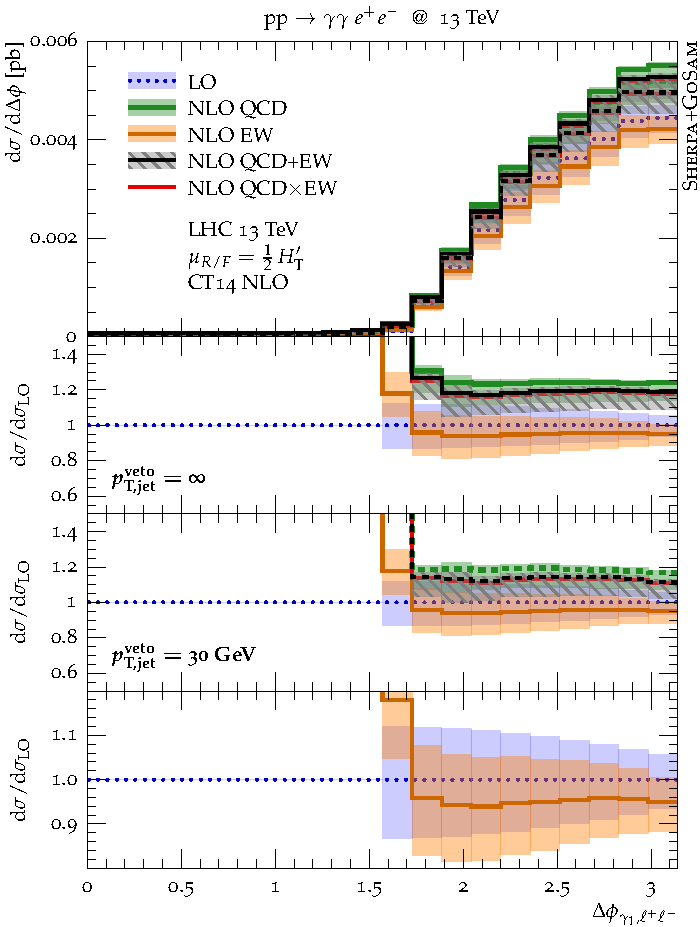
\includegraphics[width=0.32\textwidth]{figs_aaz/dphi_y1_l1l2}
  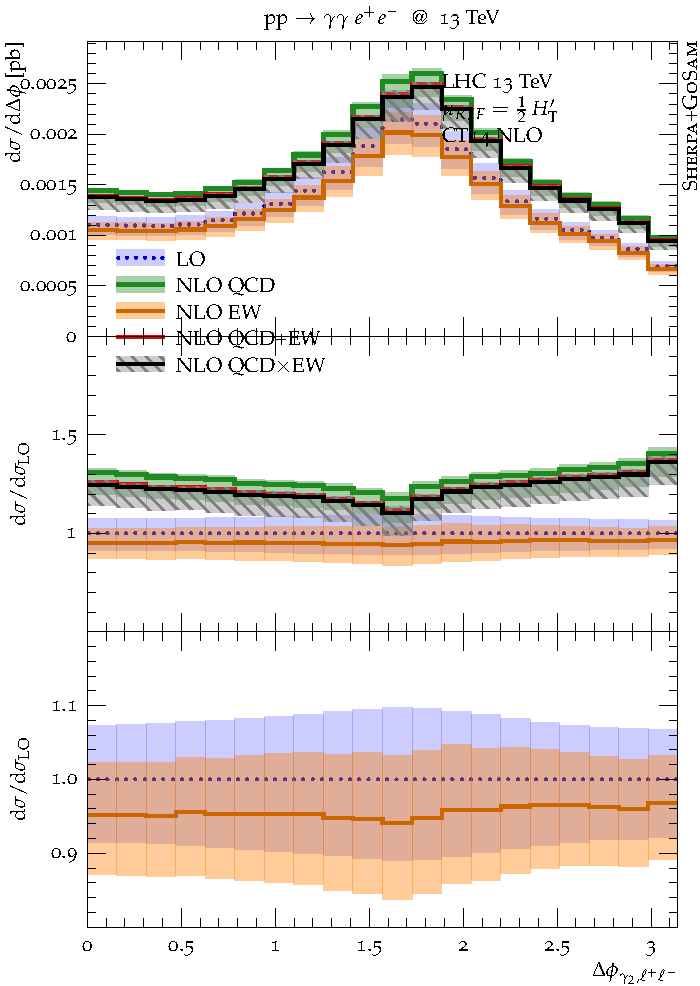
\includegraphics[width=0.32\textwidth]{figs_aaz/dphi_y2_l1l2}
  \caption{
    Azimuthal separation of the leading and subleading photon (left),
    the leading photon and the lepton pair (centre), and the subleading 
    photon and the lepton pair (right)
    in diple photon production in association with a lepton pair 
    at the LHC at 13\,TeV. 
    Details as in Fig.\ \ref{fig:aaa:pt}.\\
    \comment{MS: Spike in $\Delta\phi_{\gamma_1,\ell_1\ell_2}$ is in NLO \QCDtEW\ 
             and comes from $\deltaEW\approx 10$ in this bin at the 
             edge of the LO phase space.}
    \label{fig:aaz:dphi}
  }
\end{figure}



\begin{figure}[t!]
  \setlength{\unitlength}{\textwidth}
  \begin{picture}(0,0.37)
    \put(0,0.24){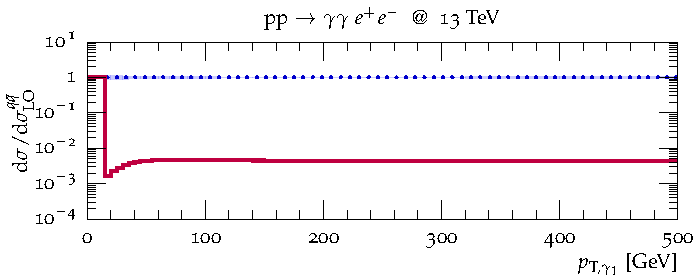
\includegraphics[width=0.32\textwidth]{figs_aaz_aa-ind/pT_y1}}
    \put(0,0.12){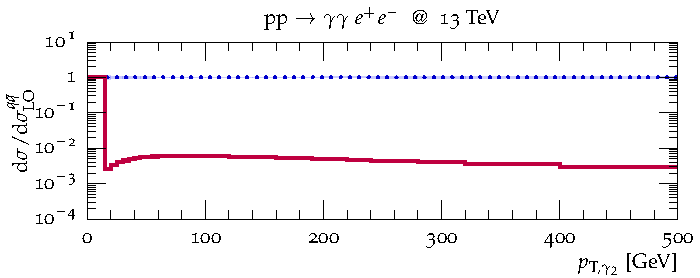
\includegraphics[width=0.32\textwidth]{figs_aaz_aa-ind/pT_y2}}
    \put(0,0){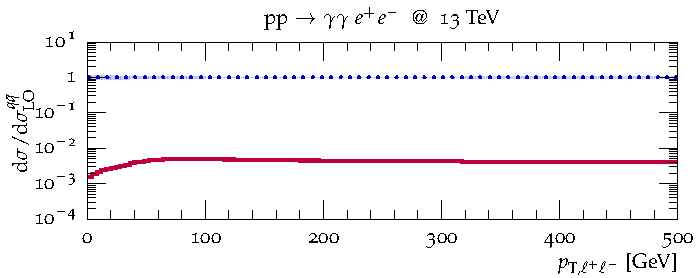
\includegraphics[width=0.32\textwidth]{figs_aaz_aa-ind/pT_l1l2_comb_log}}
    \put(0.33,0.24){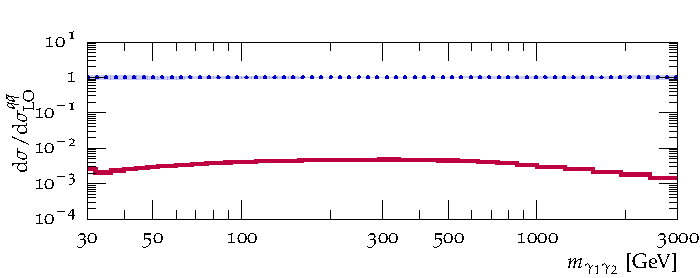
\includegraphics[width=0.32\textwidth]{figs_aaz_aa-ind/m_y1y2_comb_log}}
    \put(0.33,0.12){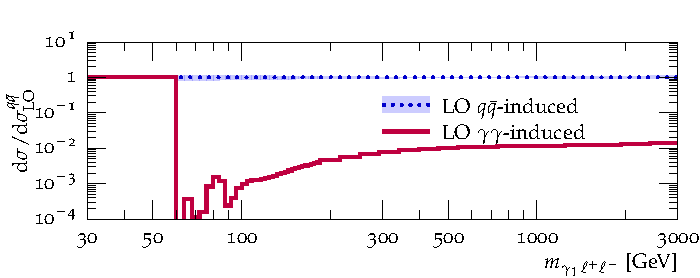
\includegraphics[width=0.32\textwidth]{figs_aaz_aa-ind/m_y1l1l2_comb_log}}
    \put(0.33,0){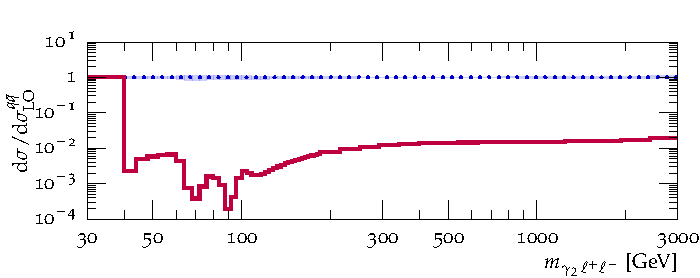
\includegraphics[width=0.32\textwidth]{figs_aaz_aa-ind/m_y2l1l2_comb_log}}
    \put(0.66,0.24){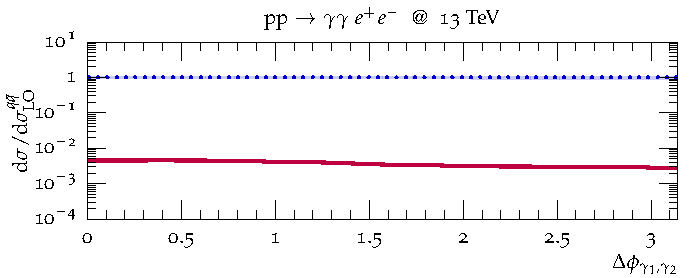
\includegraphics[width=0.32\textwidth]{figs_aaz_aa-ind/dphi_y1_y2}}
    \put(0.66,0.12){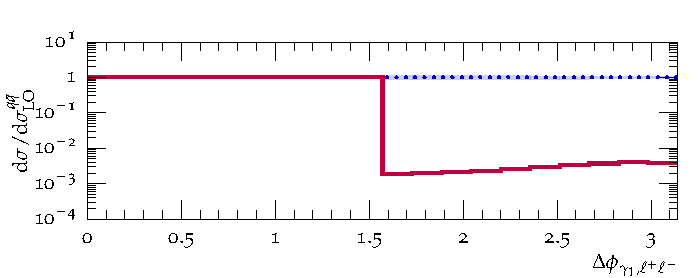
\includegraphics[width=0.32\textwidth]{figs_aaz_aa-ind/dphi_y1_l1l2}}
    \put(0.66,0){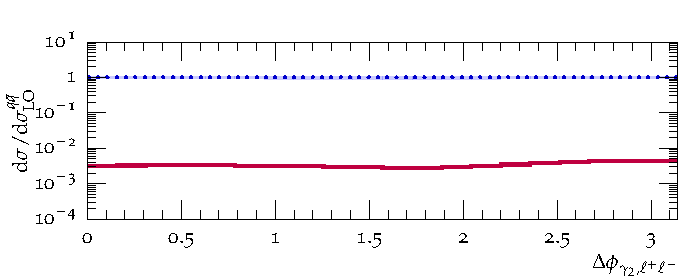
\includegraphics[width=0.32\textwidth]{figs_aaz_aa-ind/dphi_y2_l1l2}}
  \end{picture}
  \caption{
    Contribution of $\gamma\gamma$-induced production channels at LO.
    \label{fig:aaz:aa-ind}
  }
\end{figure}


